\chapter{Results}

\section{TDC}
The TDC was simulated in Cadence Virtuoso using the Spectre simulator. The test bench (TB) is that of figure \ref{fig:TB_TDC_Schematic}, where the reference input signal is connected
to a square wave voltage source with a frequency of 100 MHz and a 50\% duty cycle, the other input (feedback) is connected to a similar source but with a frequency of either 100.1 MHz
or 99.9 MHz depending on whether a positive or negative phase difference is to be measured. Both of these cases simulate conditions that would occur in a PLL when the DCO frequency is
slightly higher or lower than the reference frequency, respectively. The outputs of the TDC are connected to a load capacitance of 5 fF to simulate the effect of the subsequent DLF.

%TB_TDC_Schematic

The transient simulation of the TDC is separated in two parts, one for the forward path TDC and the other for the backward path TDC. Figures \ref{fig:TDC_TRAN_fwd} and \ref{fig:TDC_TRAN_bwd} show
the transient simulation results for the forward and backward path TDCs, respectively. The top two waveforms are the reference and feedback input signals, while the bottom waveforms are the TDC outputs.
The simulation is run for a total of 1.9 $\mu$s, where the first 0.3 $\mu$s is a settling time to allow the DLL to reach a steady state before measurements are taken. The next 1.6 $\mu$s are used for measurements,
allowing 10 cycles for each code.

\begin{figure}[H]
    \centering
    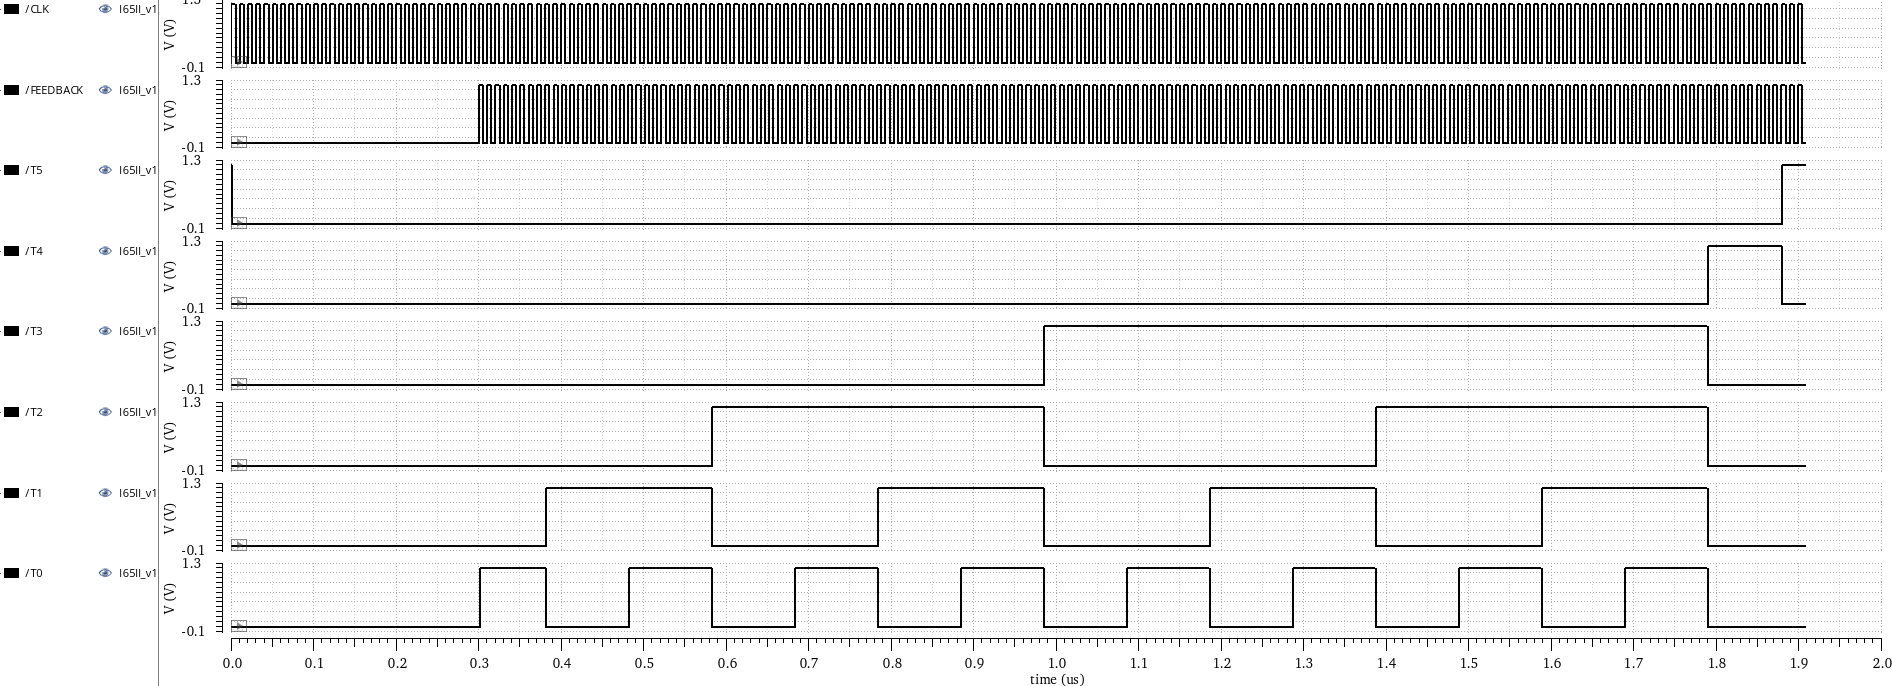
\includegraphics[width=1\textwidth]{figures/TDC_TRAN_fwd.png}
    \caption{Transient simulation results for the forward path (TT).}
    \label{fig:TDC_TRAN_fwd}
\end{figure}

\begin{figure}[H]
    \centering
    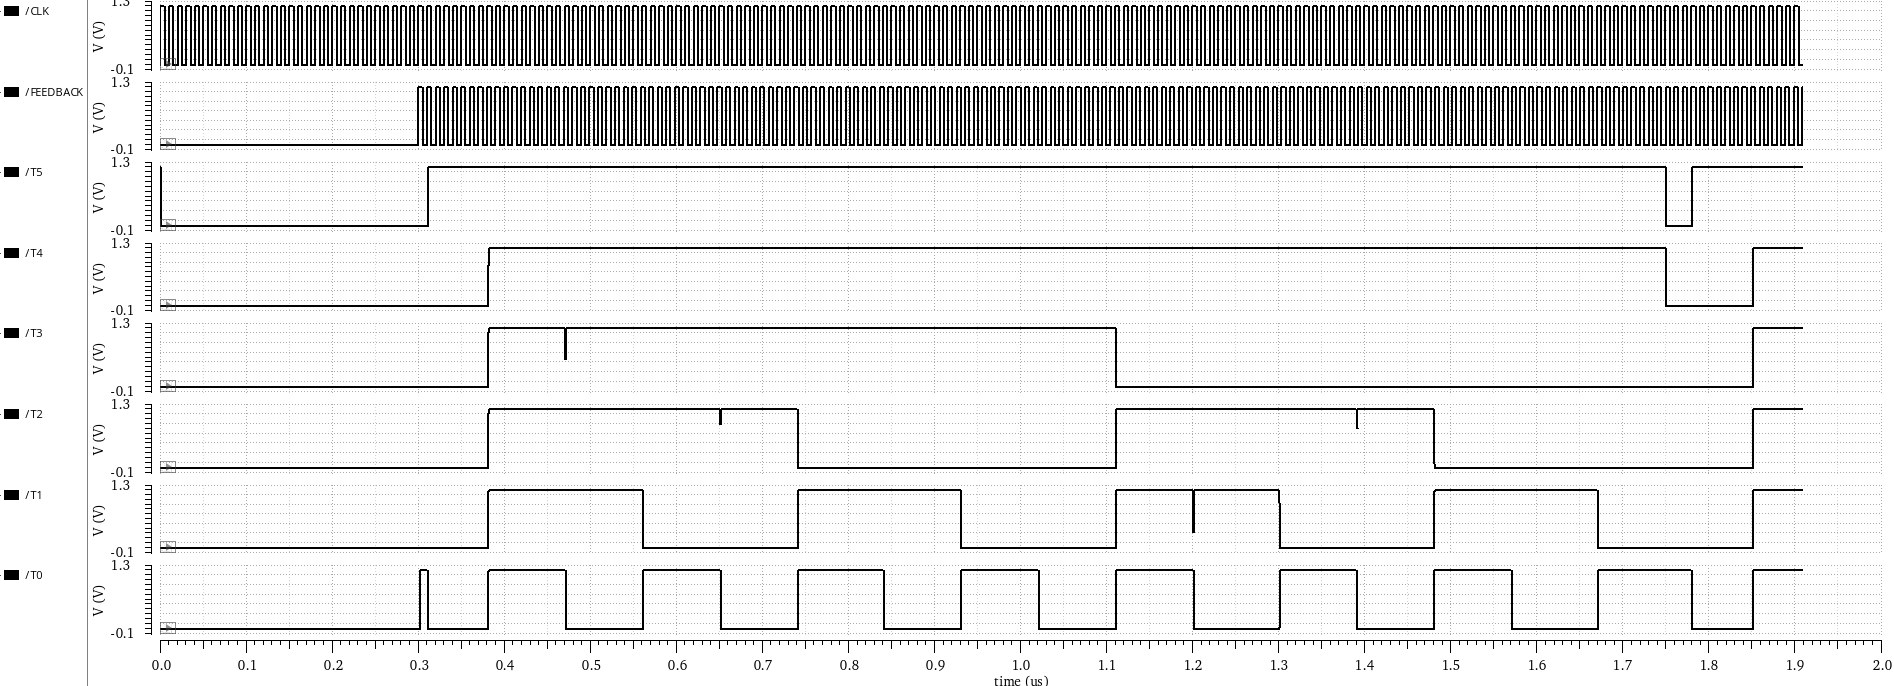
\includegraphics[width=1\textwidth]{figures/TDC_TRAN_bwd.png}
    \caption{Transient simulation results for the backward path (TT).}
    \label{fig:TDC_TRAN_bwd}
\end{figure}

The measured conversion time (defined in chapter 2 as the minimum time required for the TDC to convert an input time interval into a digital word) is found to be 687.5 ps for the typical corner (TT). From the
transient results the output characteristic of the TDC can be extracted by measuring the output code at a given delay time between the reference and feedback signals.

The output characteristic of the TDC for the typical corner is shown in figure \ref{fig:TDC_Transfer_Characteristic}, where the output is seen to increase linearly with the phase difference between the
reference and feedback signals. The red blue line is the actual output characteristic while the red dotted line is the best straight line fit. The TDC is seen to have a resolution of 617.5 ps and a dynamic
range of 19.687 ns. Notice that this is very similar to a PFD with a maximum phase difference of almost two full cycles but without a dead zone.

\begin{figure}[H]
    \centering
    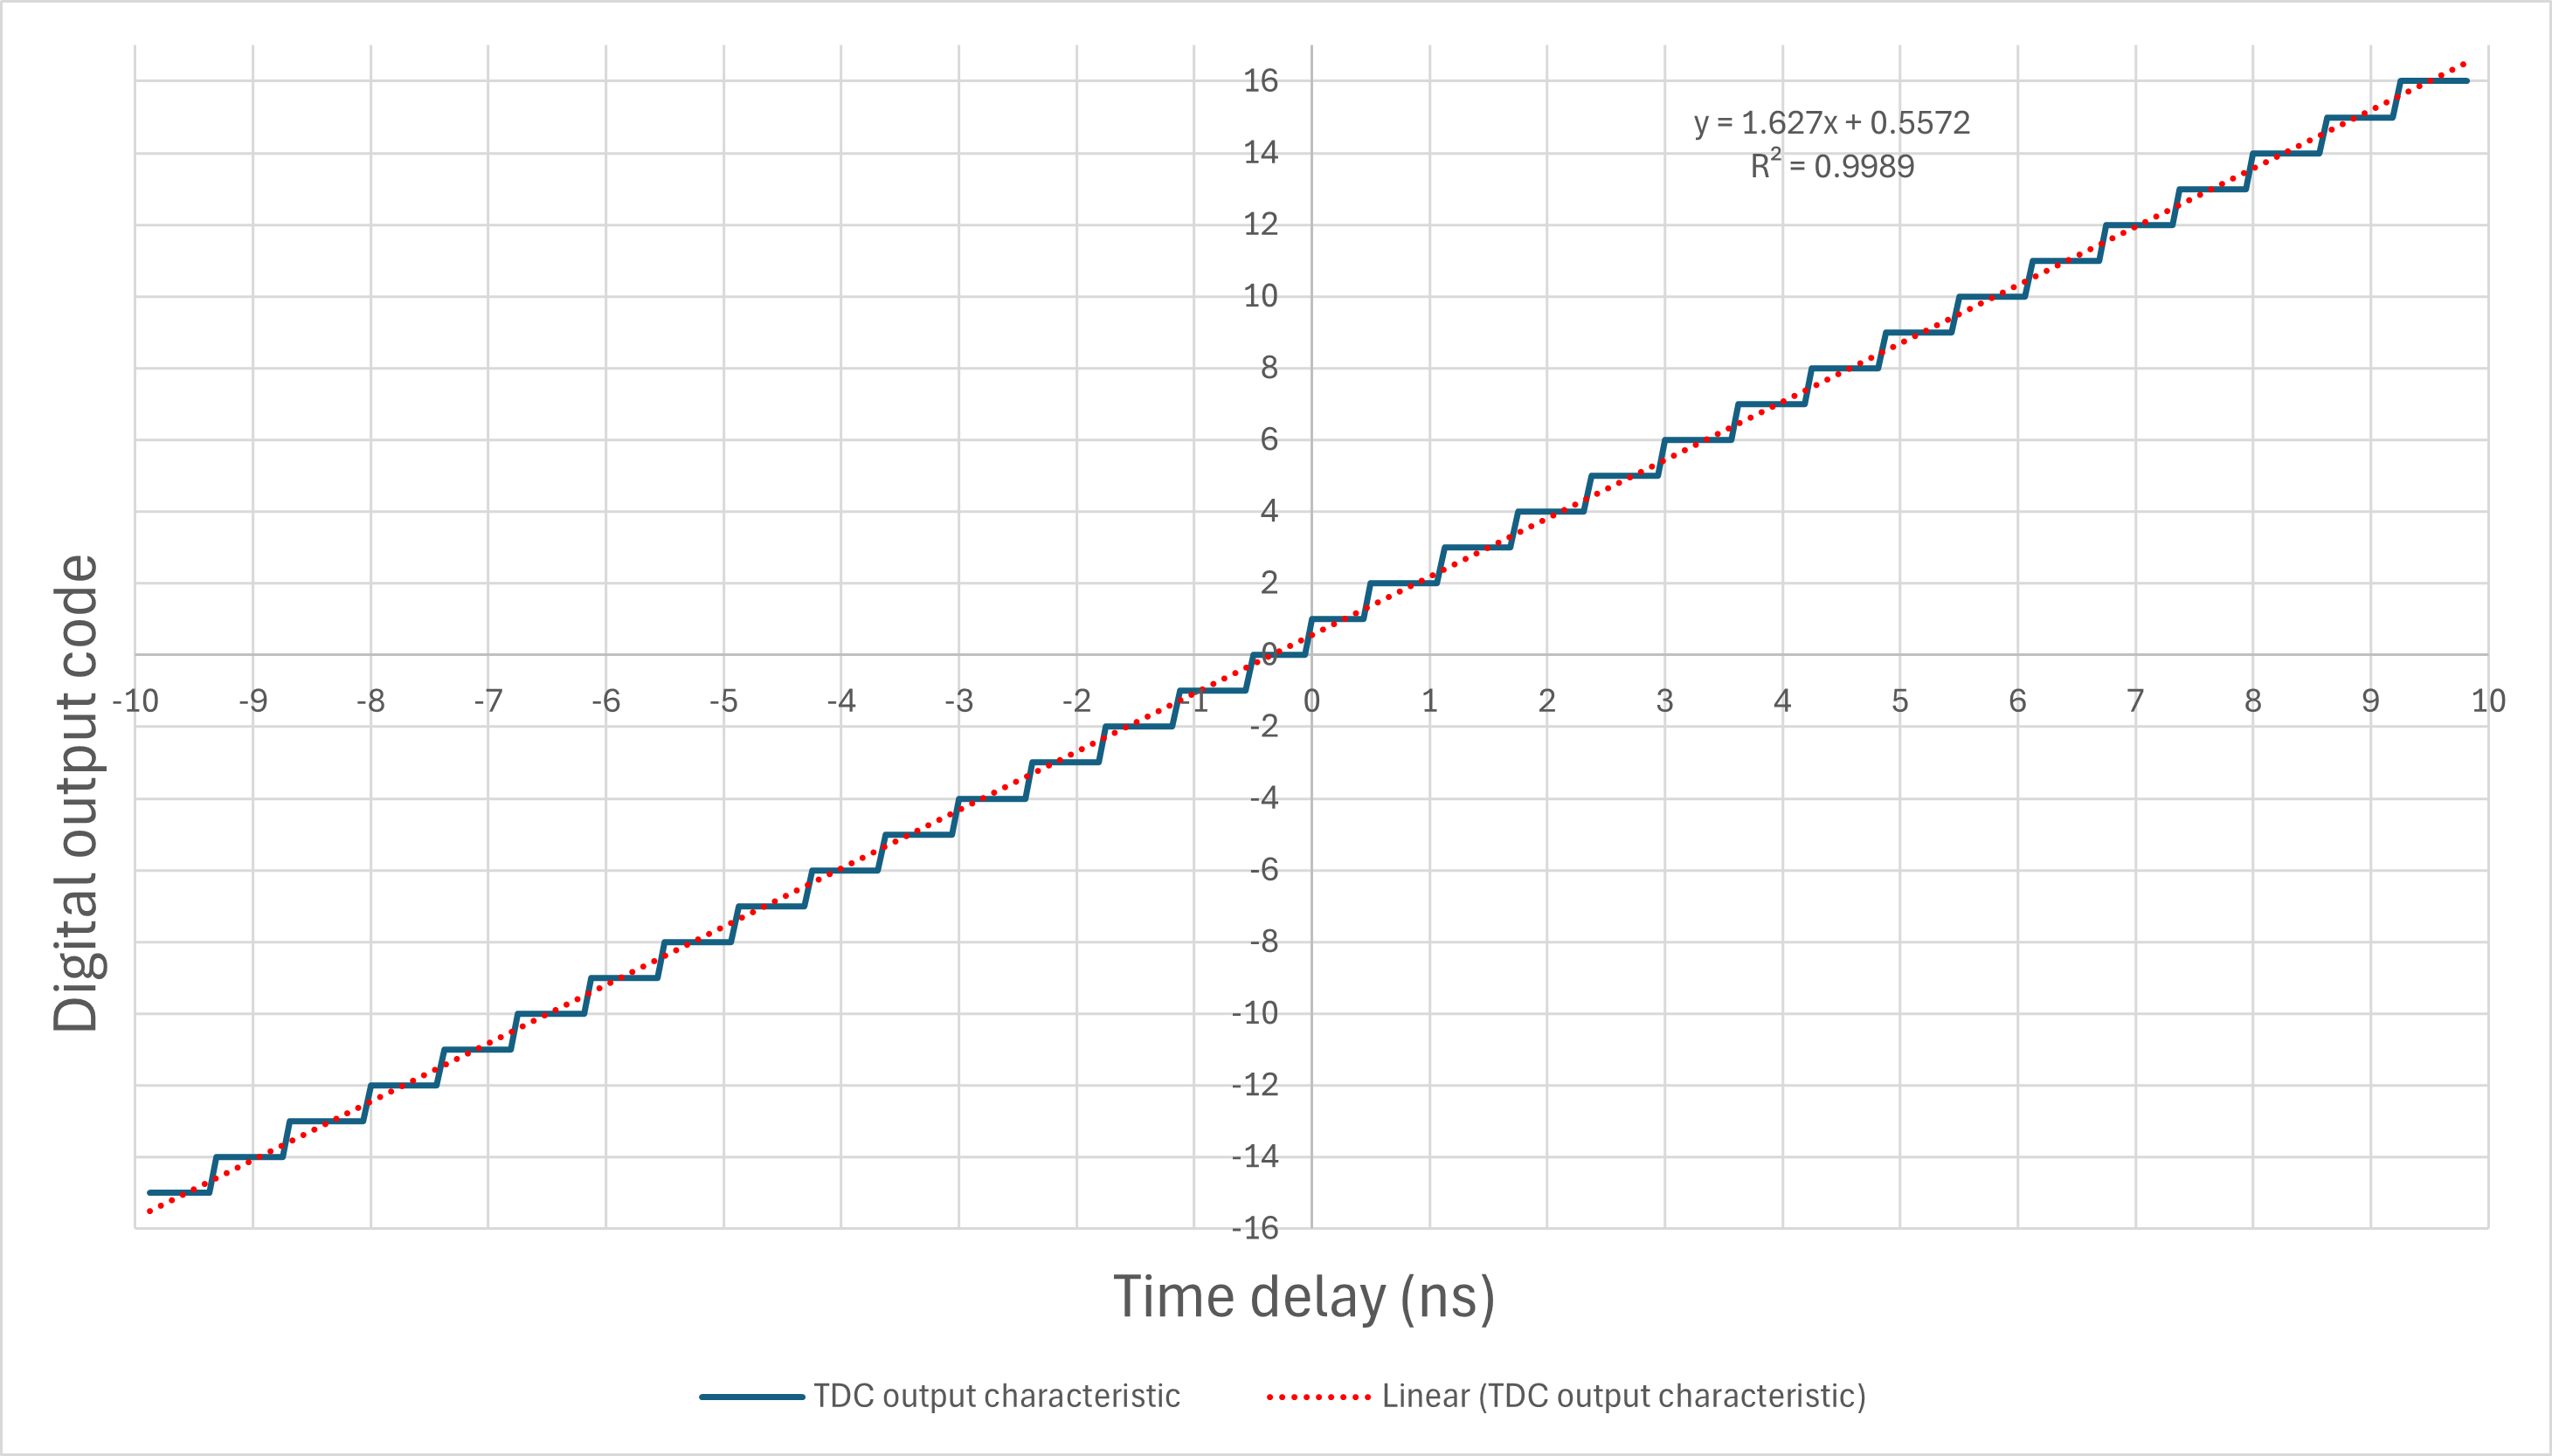
\includegraphics[width=1\textwidth]{figures/TDC_output_characteristic_result.png}
    \caption{TDC Transfer Characteristic for the TT corner.}
    \label{fig:TDC_Transfer_Characteristic}
\end{figure}

From the output characteristic, the gain of the TDC can be calculated as the slope of the best fit line, which is found to be 1.627. The linearity is calculated with the best straight line fit method,
arriving at a DNL of -0.11 LSB and INL of 0.39 LSB.

\section{DCO}

\noindent\rule{\textwidth}{1pt}